\section{Sistema de Monitoreo Remoto de Pacientes}

\subsection{Introducción}

\subsubsection{Antecedentes}
El Monitoreo Remoto de Pacientes ha emergido como una tecnología para mejorar la atención médica moderna, permitiendo la vigilancia continua del paciente fuera de los entornos clínicos tradicionales. 
Sin embargo, estos sistemas enfrentan desafíos en el mantenimiento de la calidad consistente de datos y la integración de mediciones de múltiples dispositivos con diferentes niveles de confiabilidad 
y tasas de muestreo.

\subsubsection{Planteamiento del Problema}
Los sistemas tradicionales de monitoreo de signos vitales frecuentemente enfrentan dificultades con:
\begin{itemize}
    \item Temporización inconsistente de mediciones entre diferentes signos vitales
    \item Variación en la confiabilidad y precisión de los dispositivos
    \item Integración de múltiples fuentes de datos para el mismo signo vital
    \item Mantenimiento de la validez clínica con datos incompletos
\end{itemize}

\subsubsection{Solución Propuesta}
Se propone abordar estos desafíos mediante:
\begin{itemize}
    \item Fusión de datos multi-dispositivo 
    \item Puntaje de calidad del dato
    \item Puntaje de frescura del dato
    \item Capacidad de degradación gradual
\end{itemize}

\subsection{Fundamento Clínico: El Sistema de Puntuación NEWS2}

\subsubsection{Descripción General de NEWS2}
El National Early Warning Score 2 (NEWS2) es una herramienta de evaluación estandarizada utilizada para detectar el deterioro clínico. Evalúa seis parámetros fisiológicos:
\begin{itemize}
    \item Frecuencia respiratoria
    \item Saturación de oxígeno
    \item Presión arterial sistólica
    \item Frecuencia cardíaca
    \item Nivel de consciencia
    \item Temperatura
\end{itemize}

\subsubsection{Desafíos de Implementación Tradicional}
NEWS2 fue originalmente diseñado para mediciones manuales periódicas en entornos clínicos. Su adaptación para monitoreo remoto continuo presenta varios desafíos:
\begin{itemize}
    \item Diferentes frecuencias de medición para diferentes parámetros
    \item Calidad y confiabilidad variable de las mediciones
    \item Necesidad de actualizaciones de puntuación en tiempo real
    \item Manejo de datos faltantes o degradados
\end{itemize}

\subsection{gdNEWS2}

\subsubsection{Concepto y Fundamentos}
Se propone aumentar el sistema NEWS2 con el concepto de degradación gradual (graceful degradation) de modo que la puntuación aún sea útil incluso cuando la medición de alguno de los datos de signos vitales no 
se encuentre presente o no se confíe del todo en la calidad del mismo.
Cada parámetro de NEWS2 tiene un puntaje de calidad y de frescura asociado, que se utilizarán para definir el nivel de confianza que se le tiene a dicho parámetro.
De esta forma, se puede calcular una puntuación de alerta temprana incluso cuando no se tienen todos los datos disponibles 
y brindarle transparencia al profesional de la salud para que tome las decisiones correspondientes en cuanto al tratamiento del paciente.

\subsection{Formato de Datos de Mediciones Brutas}

Los datos serán recibidos en formato JSON, con un esquema común para todos los tipos de mediciones.
El esquema general es el siguiente:
\begin{lstlisting}[
    frame=single,
    numbers=left,
    numbersep=5pt,
    xleftmargin=20pt,
    language=JSON,
    basicstyle=\ttfamily,
    commentstyle=\color{gray},
    caption={JSON example},
    label={json-example}]
{
    "measurement_type": "RESPIRATORY_RATE" | "HEART_RATE" | "OXYGEN_SATURATION" | "BLOOD_PRESSURE_SYSTOLIC" | "TEMPERATURE" | "CONSCIOUSNESS",
    "measurement_timestamp": "datetime",
    "device_id": "string",
    "raw_value": "number",
    "battery": "number",
    "signal_strength": "number"
}
\end{lstlisting}
\newpage

\subsection{Algoritmo de Puntuación de Calidad}
Un nuevo algoritmo de puntuación de calidad debería basarse en la experiencia clínica y la evidencia científica. Para el caso de estudio presentado, 
se propone un algoritmo sencillo a fin de ilustrar su potencial y mantener limitado el enfoque de este trabajo.

Se tomarán los identificadores de los dispositivos, que luego serán clasificados en 3 grupos cada uno con un peso asociado: 
\begin{itemize}
    \item Dispositivos de calidad médica: 1.0
    \item Dispositivos de calidad premium: 0.7
    \item Dispositivos de calidad de consumo: 0.4
\end{itemize}

Además, se tomará en cuenta la señal de batería y la intensidad de la señal, que serán clasificados en 3 grupos cada uno con un peso asociado:
\begin{itemize}
    \item Batería a mas del 80\%: 1.0
    \item Batería entre 80\% y 50\%: 0.7
    \item Batería entre 50\% y 20\%: 0.6
    \item Batería a menos de 20\%: 0.4
\end{itemize}

Por último, se tomará en cuenta la intensidad de la señal:
\begin{itemize}
    \item Valor de señal de mas de 0.8: 1.0
    \item Valor de señal entre 0.8 y 0.6: 0.8
    \item Valor de señal entre 0.5 y 0.6: 0.6
    \item Valor de señal menor a 0.5: 0.4
\end{itemize}

De esta manera, el cálculo de la puntuación de calidad se realizará de la siguiente manera:


\begin{equation}
    \text{Quality Score} = 0.7 \times \text{Device Quality} + 0.2 \times \text{Battery Quality} + 0.1 \times \text{Signal Quality}
\end{equation}


En este momento, los valores tanto de los pesos como de los parametros son arbitrarios y se espera que en caso de encontrar útil este acercamiento, 
futuras iteraciones ajusten estos parámetros o utilicen un criterio diferente para su cálculo.

\subsection{Algoritmo de Puntuación de Frescura}

Para medir la frescura de los datos, se propone un enfoque simple que considera el tiempo transcurrido desde la última medición 
y el tiempo que le tomó a la medición actual llegar a ser procesada.

Tiempo desde medición hasta procesamiento:
\begin{itemize}
    \item Menos de una hora: 1.0
    \item Entre una y seis horas: 0.9
    \item Entre seis y doce horas: 0.7
    \item Entre doce y veinticuatro horas: 0.5
    \item Entre veinticuatro y cuarenta y ocho horas: 0.3
    \item En cualquier otro caso: 0.2
\end{itemize}

Tiempos entre mediciones:
\begin{itemize}
    \item Menos de cuatro horas: 1.0
    \item Entre cuatro y ocho horas: 0.8
    \item Entre ocho y doce horas: 0.6
    \item Entre doce y veinticuatro horas: 0.4
    \item Más de veinticuatro horas: 0.2
\end{itemize}

De esta manera, se propone el siguiente algoritmo de puntuación de frescura:

\begin{equation}
    \text{Freshness Score} = 0.5 \times \text{Time Since Last Measurement} + 0.5 \times \text{Time Since Measurement}
\end{equation}

\subsection{Algoritmo de Puntuación de Degradación}

Este algoritmo se encargará de calcular la puntuación de degradación de la puntuación NEWS2 en caso de que no se tengan todos los datos disponibles.
Simboliza la confianza que se le tiene a la puntuación NEWS2 en base a la calidad y frescura de los datos.

Se propone utilizar la siguiente fórmula para calcular la puntuación de degradación:

\begin{equation}
    \text{Degradation Score} = 0.7 \times \text{Quality Score} + 0.3 \times \text{Freshness Score}
\end{equation}

Se calcula este puntaje para cada uno de los parámetros de NEWS2 y se promedia para obtener la puntuación de degradación final.

\subsection{Algoritmo de Puntuación de NEWS2}

El algoritmo de puntuación NEWS2 se basa en la suma de los puntajes de cada uno de los parámetros,
\begin{equation}
    \text{NEWS2 Score} = \sum_{i=1}^{n} \text{Parameter Score}_i
\end{equation}
donde $n$ es la cantidad de parámetros que se tienen disponibles.
En caso de que no se tenga un parámetro disponible, se asumirá una puntuación de cero para ese parámetro en su lugar.
De esta manera, se puede calcular la puntuación NEWS2 incluso cuando no se tienen todos los datos disponibles.

Por otro lado, se propone utilizar la puntuación de degradación para dar contexto sobre la puntuación NEWS2 final.
Así, se puede explicar que tan confiable es la puntuación NEWS2 calculada en base a los datos disponibles.

\subsection{Pipeline de Procesamiento}
El pipeline de procesamiento se encargará de recibir los datos en formato JSON,
realizar el procesamiento de los mismos y devolver la puntuación NEWS2 calculada.

Esto se realizará de la siguiente manera:
\begin{itemize}
    \item Recepción de datos en formato JSON
    \item Enriquecimiento de los datos con los puntajes de calidad y frescura
    \item Enrutamiento de los datos para su procesamiento particular según el signo vital
    \item Cálculo de la puntuación NEWS2 para cada una de las Componentes
    \item Unión y agrupación según una ventana de tiempo
    \item Calculo de valores de agregación de los puntajes de NEWS2 y de degradación
\end{itemize}

A continuación se presenta un diagrama de flujo del pipeline de procesamiento:
\begin{figure}[h]
    \centering
    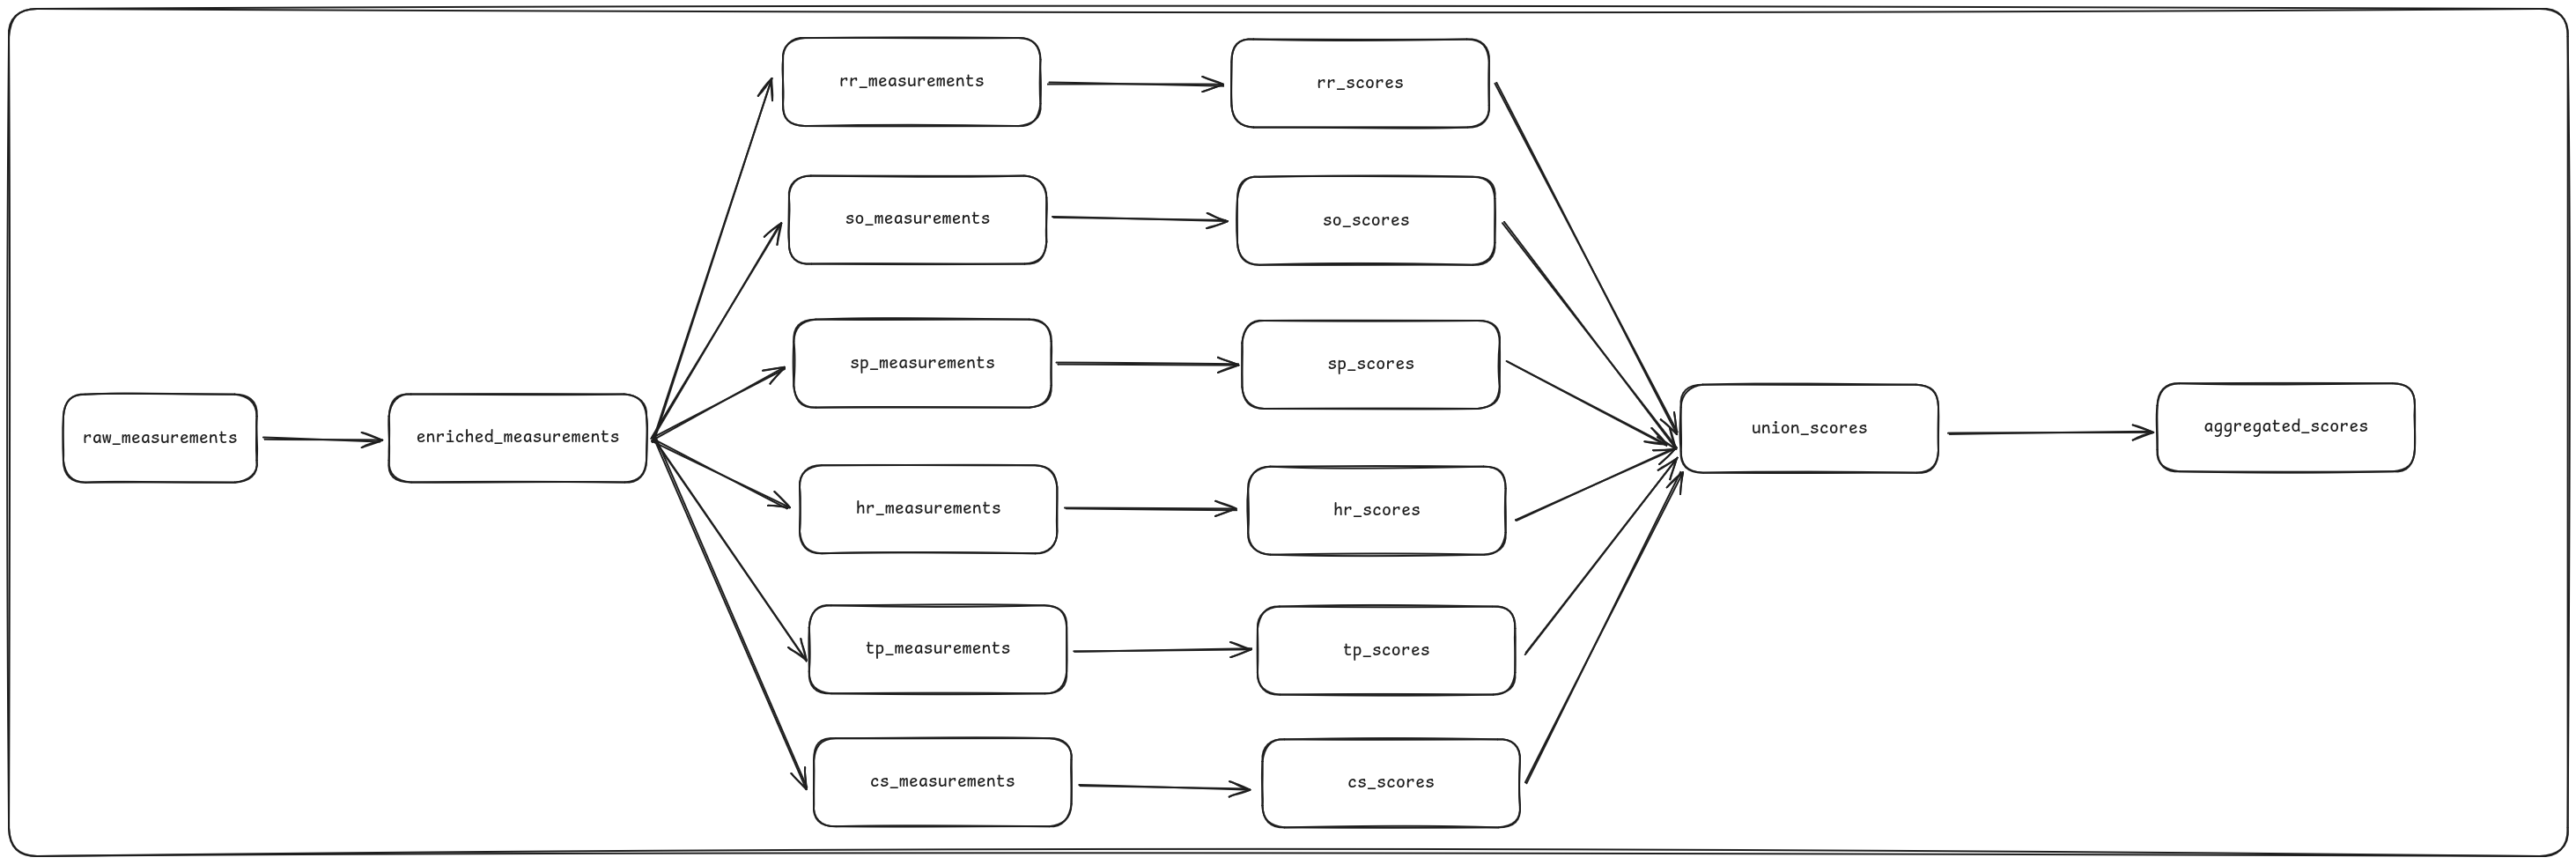
\includegraphics[width=1\textwidth]{desarrollo/pipeline.png}
    \caption{Diagrama de flujo del pipeline de procesamiento}
    \label{fig:flowchart}
\end{figure}